\documentclass[aspectratio=169,13pt,t] {beamer}
%
% Choose how your presentation looks.
%
% For more themes, color themes and font themes, see:
% http://deic.uab.es/~iblanes/beamer_gallery/index_by_theme.html
%
\mode<presentation>
{
  \usetheme{Madrid}      % or try Darmstadt, Madrid, Warsaw, ...
  \usecolortheme{beaver} % or try albatross, beaver, crane, ...
  \usefonttheme{serif}  % or try serif, structurebold, ...
%  \setbeamertemplate{navigation symbols}{}
  \setbeamertemplate{caption}[numbered]
  \setbeamertemplate{items}[default]
} 

\usepackage[,UTF8,linespread=1.2]{ctex}
\usepackage{wrapfig}
\usepackage{caption}
\captionsetup[figure]{name=图,labelsep=period}
\usepackage[,most]{tcolorbox}
\usepackage{picinpar}
\usetikzlibrary{arrows.meta}


\usepackage{xcolor}
\definecolor{xy_blue}{cmyk}{0.6,0.35,0.0,0.4}
\definecolor{xy_orange}{cmyk}{0.0,0.7,1.0,0.0}
\definecolor{xy_green}{cmyk}{0.2,0.0,1.0,0.15}
\xdefinecolor{xy_gold}{RGB}{135,103,79}
\xdefinecolor{xy2_gold}{cmyk}{0,0.35,0.75,0.05}


\setbeamercolor{section number projected}{fg=red,bg=red!20}%控制球的颜色
\setbeamercolor{subsection number projected}{fg=blue,bg=blue!40}
\setbeamercolor{item}{fg=xy_gold} %设置列表项颜色

\usepackage{amsthm}
\newtheorem{peroration}{结论：}
\newtheorem{exploration}{探究：}
\newtheorem{prooft}{证明：}
\newtheorem{question}{问题}
\newtheorem*{solve}{解:} 
\newtheorem{instance}{例}   % 解：独立计数器
\BeforeBeginEnvironment{peroration}{%
	\setbeamercolor{block title}{bg=xy_green,fg=white}
	\setbeamercolor{block body}{bg=xy_green!10}
}
\AfterEndEnvironment{peroration}{
	\setbeamercolor{block title}{bg=xy_blue,fg=white}
	\setbeamercolor{block body}{bg=xy_blue!10}
}
\BeforeBeginEnvironment{exploration}{%
	\setbeamercolor{block title}{bg=xy_orange,fg=white}
	\setbeamercolor{block body}{bg=xy_orange!10}
}
\AfterEndEnvironment{peroration}{
	\setbeamercolor{block title}{bg=xy_blue,fg=white}
	\setbeamercolor{block body}{bg=xy_blue!10}
}
\BeforeBeginEnvironment{solution}{%
	\setbeamercolor{block title}{bg=xy_green,fg=white}
	\setbeamercolor{block body}{bg=xy_green!10}
}
\AfterEndEnvironment{solution}{
	\setbeamercolor{block title}{bg=xy_green,fg=white}
	\setbeamercolor{block body}{bg=xy_green!10}
}
\BeforeBeginEnvironment{prooft}{%
	\setbeamercolor{block title}{bg=xy_green,fg=white}
	\setbeamercolor{block body}{bg=xy_green!10}
}
\AfterEndEnvironment{prooft}{
	\setbeamercolor{block title}{bg=xy_green,fg=white}
	\setbeamercolor{block body}{bg=xy_green!10}
}
\BeforeBeginEnvironment{question}{%
	\setbeamercolor{block title}{bg=xy_orange,fg=white}
	\setbeamercolor{block body}{bg=xy_orange!10}
}
\AfterEndEnvironment{question}{
	\setbeamercolor{block title}{bg=xy_green,fg=white}
	\setbeamercolor{block body}{bg=xy_green!10}
}
\BeforeBeginEnvironment{solve}{%解：
	\begingroup
	\setbeamercolor{block title}{bg=xy_orange!60,fg=white}
	\setbeamercolor{block body}{bg=xy_orange!10}
}
\AfterEndEnvironment{solve}{%解：
	\endgroup
}

\setbeamercolor{prooft}{fg=red, bg=green!10}       % 标题颜色
\setbeamercolor{prooft body}{fg=red, bg=red!5}  % 内容块背景
\setbeamerfont{prooft head}{series=\bfseries}       % 标题字体
\setbeamerfont{question body}{shape=\upshape}         % 内容字体
\renewcommand{\thefigure}{\arabic{figure}}

\newtcolorbox{summarybox}[1][]{
	colback=purple!10,
	colframe=purple!70!black,
	fonttitle=\bfseries,
	title=#1,
	arc=1mm,
	boxrule=0pt,drop shadow,
	left=2mm, right=2mm, top=2mm, bottom=2mm,
}
\newtcolorbox{summarybox-answer}{
	width=0.9\textwidth,
	colback=white,
	blanker,
	borderline west={2pt}{20pt}{cyan},
	left=10mm, right=2mm, top=2mm, bottom=2mm,
	}
\title[3.1.1函数的概念（二）]{3.1.1函数的概念（二）}
\subtitle{区间、定义域与同一函数}
\author[好好学习，努力向上]{}
\institute{}
\date{2026.10.12}
%\setbeamertemplate{theorems}[numbered]
\theoremstyle{definition}
\newtheorem{exam}{例}
\AtBeginSection[]
{
  \begin{frame}<beamer>
    \frametitle{本节主要内容}
    \tableofcontents[currentsection,currentsubsection]
  \end{frame}
}

\AtBeginDocument{
	\setlength{\abovedisplayskip}{3pt}
	\setlength{\belowdisplayskip}{3pt}
	\setbeamertemplate{theorems}[numbered]
}

\begin{document}
\begin{frame}{}
	\titlepage
\end{frame}

\begin{frame}{内容概览}
	\tableofcontents
\end{frame}

\section{区间的概念}

\begin{frame}{区间的引入}
	\begin{question}
	研究函数时常会用到区间的概念.
	
	设 \(a, b\) 是两个实数，而且 \(a < b\). 我们规定：
	\end{question}
	\pause
	\begin{itemize}
		\item 满足不等式 \(a \leqslant x \leqslant b\) 的实数 \(x\) 的集合叫做\textbf{闭区间}，表示为 \([a, b]\)；
		\item 满足不等式 \(a < x < b\) 的实数 \(x\) 的集合叫做\textbf{开区间}，表示为 \((a, b)\)；
		\item 满足不等式 \(a \leqslant x < b\) 或 \(a < x \leqslant b\) 的实数 \(x\) 的集合叫做\textbf{半开半闭区间}，分别表示为 \([a, b)\)，\((a, b]\).
	\end{itemize}
	\pause
	\begin{summarybox-answer}
		这里的实数 \(a\) 与 \(b\) 都叫做相应区间的\textbf{端点}.
	\end{summarybox-answer}
\end{frame}

%\begin{frame}{区间的数轴表示}
%	\begin{table}[h]
%		\centering	
%		\renewcommand{\arraystretch}{1.5}
%		
%		\begin{tabular}{|c|c|}
%			\hline
%			\textbf{区间} & \textbf{数轴表示} \\ \hline
%			\([a, b]\)（闭区间） & \(\bullet\!\!-\!\!\!-\!\!\!-\!\!\!-\!\!\!-\!\!\circ\) 不对，见下 \\ \hline
%			\((a, b)\)（开区间） & 空心端点 \\ \hline
%			\([a, b)\) & 左闭右开 \\ \hline
%			\((a, b]\) & 左开右闭 \\ \hline
%		\end{tabular}
%	\end{table}
%	\pause
%	\begin{summarybox-answer}
%		在数轴表示时，用\textbf{实心点}表示包括在区间内的端点，用\textbf{空心点}表示不包括在区间内的端点.
%	\end{summarybox-answer}
%\end{frame}

\begin{frame}{有限区间}
	设 \(a,b\) 是两个实数，且 \(a<b\). 规定：
	\small
	\begin{center}
		\renewcommand{\arraystretch}{1.35}
		\begin{tabular}{|c|c|c|c|}
			\hline
			\textbf{名称} & \textbf{集合} & \textbf{记号} & 数轴表示\\ \hline
			闭区间 & \(\{x\mid a\le x\le b\}\) & \([a,\,b]\) & 
			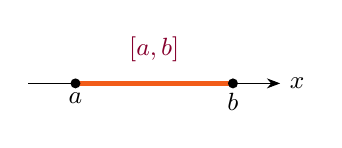
\begin{tikzpicture}[>=Stealth, baseline=-0.6ex]
				% closed [a,b]
				\draw[->] (0,0) -- (3.2,0) node[right]{\small \(x\)};
				\draw[ultra thick, xy_orange] (0.6,0) -- (2.6,0);
				\fill (0.6,0) circle (1.8pt); 
				\fill (2.6,0) circle (1.8pt);
				\node[below] at (0.6,0){\small \(a\)}; \node[below] at (2.6,0){\small \(b\)};
				\node[above, purple!70!black] at (1.6,0.15){\small \([a,b]\)};
			\end{tikzpicture}\\ \hline
			开区间 & \(\{x\mid a< x< b\}\) & \((a,\,b)\) & 	
			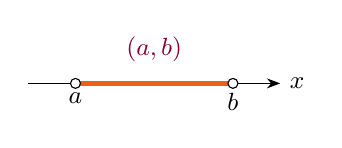
\begin{tikzpicture}[>=Stealth, baseline=-0.6ex]
				\draw[->] (0,0) -- (3.2,0) node[right]{\small \(x\)};
				\draw[ultra thick, xy_orange] (0.6,0) -- (2.6,0);
				\filldraw[fill=white, draw=black] (0.6,0) circle (1.8pt); 
				\filldraw[fill=white, draw=black] (2.6,0) circle (1.8pt);
				\node[below] at (0.6,0){\small \(a\)}; 
				\node[below] at (2.6,0){\small \(b\)};
				\node[above, purple!70!black] at (1.6,0.15){\small \((a,b)\)};
			\end{tikzpicture}\\ \hline
			半开半闭 & \(\{x\mid a\le x< b\}\) & \([a,\,b)\) &    
			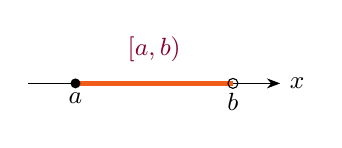
\begin{tikzpicture}[>=Stealth, baseline=-0.6ex]
				% closed [a,b]
				\draw[->] (0,0) -- (3.2,0) node[right]{\small \(x\)};
				\draw[ultra thick, xy_orange] (0.6,0) -- (2.6,0);
				\fill (0.6,0) circle (1.8pt); 
				\draw (2.6,0) circle (1.8pt);
				\node[below] at (0.6,0){\small \(a\)}; 
				\node[below] at (2.6,0){\small \(b\)};
				\node[above, purple!70!black] at (1.6,0.15){\small \([a,b)\)};
			\end{tikzpicture}\\ \hline
			半开半闭 & \(\{x\mid a< x\le b\}\) & \((a,\,b]\) & 
			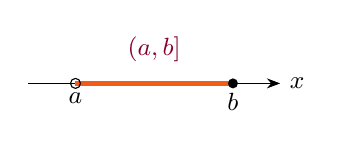
\begin{tikzpicture}[>=Stealth, baseline=-0.6ex]
				% closed [a,b]
				\draw[->] (0,0) -- (3.2,0) node[right]{\small \(x\)};
				\draw[ultra thick, xy_orange] (0.6,0) -- (2.6,0);
				\draw (0.6,0) circle (1.8pt); 
				\fill (2.6,0) circle (1.8pt);
				\node[below] at (0.6,0){\small \(a\)}; 
				\node[below] at (2.6,0){\small \(b\)};
				\node[above, purple!70!black] at (1.6,0.15){\small \((a,b]\)};
			\end{tikzpicture}\\ \hline
		\end{tabular}
	\end{center}
	\normalsize
	\vspace{0.3em}
	
\end{frame}

\section{无穷区间}

\begin{frame}{无穷区间}
		\begin{question}
		实数集 \(\mathbf{R}\) 可以用区间表示为 \((-\infty, +\infty)\)，``\(\infty\)'' 读作``无穷大''，``\(-\infty\)'' 读作``负无穷大''，``\(+\infty\)'' 读作``正无穷大''.
	\end{question}
\end{frame}

\begin{frame}{无穷区间}

	满足 \(x \geqslant a\)，\(x > a\)，\(x \leqslant b\)，\(x < b\) 的实数 \(x\) 的集合，可以用区间分别表示为：
	\begin{center}
		\renewcommand{\arraystretch}{1.35}
		\begin{tabular}{|c|c|c|}
			\hline
			\textbf{集合} & \textbf{区间} & 区间表示\\ \hline
			\(\{x\mid x\ge a\}\) & \([a,\,+\infty)\) & 
			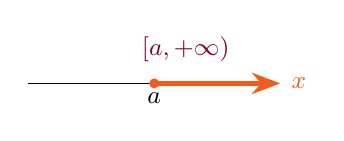
\begin{tikzpicture}[>=Stealth, baseline=-0.6ex]
				% closed [a,b]
				\draw[] (0,0) -- (1.6,0) ;
				\draw[ultra thick, xy_orange,->] (1.6,0) -- (3.2,0)node[right]{\small \(x\)};
				\fill[xy_orange] (1.6,0) circle (1.8pt); 
				\node[below] at (1.6,0){\small \(a\)}; 
				\node[above, purple!70!black] at (2,0.15){\small \([a,+\infty)\)};
			\end{tikzpicture}\\ \hline
			\(\{x\mid x> a\}\) & \((a,\,+\infty)\) & 
			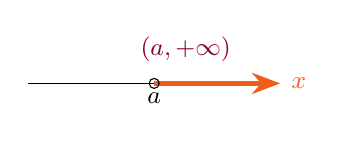
\begin{tikzpicture}[>=Stealth, baseline=-0.6ex]
				% closed [a,b]
				\draw[] (0,0) -- (1.6,0) ;
				\draw[ultra thick, xy_orange,->] (1.6,0) -- (3.2,0)node[right]{\small \(x\)};
				\draw[] (1.6,0) circle (1.8pt); 
				\node[below] at (1.6,0){\small \(a\)}; 
				\node[above, purple!70!black] at (2,0.15){\small \((a,+\infty)\)};
			\end{tikzpicture}\\ \hline
			\(\{x\mid x\le b\}\) & \((-\infty,\,b]\) & 
			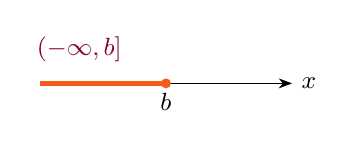
\begin{tikzpicture}[>=Stealth, baseline=-0.6ex]
				% closed [a,b]
				\draw[ultra thick, xy_orange] (0,0) -- (1.6,0) ;
				\draw[->] (1.6,0) -- (3.2,0)node[right]{\small \(x\)};
				\fill[xy_orange] (1.6,0) circle (1.8pt); 
				\node[below] at (1.6,0){\small \(b\)}; 
				\node[above, purple!70!black,] at (0.5,0.15){\small \((-\infty,b]\)};
			\end{tikzpicture}\\ \hline
			\(\{x\mid x< b\}\) & \((-\infty,\,b)\) &
			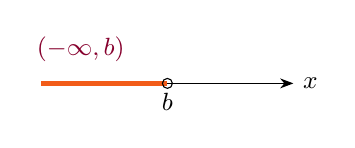
\begin{tikzpicture}[>=Stealth, baseline=-0.6ex]
				% closed [a,b]
				\draw[ultra thick, xy_orange] (0,0) -- (1.6,0) ;
				\draw[->] (1.6,0) -- (3.2,0)node[right]{\small \(x\)};
				\draw[] (1.6,0) circle (1.8pt); 
				\node[below] at (1.6,0){\small \(b\)}; 
				\node[above, purple!70!black,] at (0.5,0.15){\small \((-\infty,b)\)};
			\end{tikzpicture} \\ \hline
		\end{tabular}
	\end{center}
\end{frame}

\begin{frame}{区间表示法小结}
	\vspace{-1.5em}
	\begin{summarybox}[区间表示法总结]
		设 \(a, b\) 是实数，且 \(a < b\)，则：
		\begin{enumerate}
			\item \([a, b] = \{x \mid a \leqslant x \leqslant b\}\)
			\item \((a, b) = \{x \mid a < x < b\}\)
			\item \([a, b) = \{x \mid a \leqslant x < b\}\)
			\item \((a, b] = \{x \mid a < x \leqslant b\}\)
			\item \([a, +\infty) = \{x \mid x \geqslant a\}\)
			\item \((-\infty, b] = \{x \mid x \leqslant b\}\)
		\end{enumerate}
	\end{summarybox}
	\vspace{-1em}
	\pause
	\begin{summarybox-answer}
		\(\infty\) 不是一个具体的数，只是一个符号，所以无穷区间的端点如果是 \(\infty\)，只能用开区间表示.
	\end{summarybox-answer}
\end{frame}

\section{函数的定义域}

\begin{frame}{例2：求函数的定义域}
	\begin{exam}
	已知函数 \(f(x) = \sqrt{x+3} + \dfrac{1}{x+2}\)，
	\begin{enumerate}[(1)]
		\item 求函数的定义域；
		\item 求 \(f(-3)\)，\(f\!\left(\dfrac{2}{3}\right)\) 的值；
		\item 当 \(a > 0\) 时，求 \(f(a)\)，\(f(a-1)\) 的值.
	\end{enumerate}
	\end{exam}
	\pause
	\begin{summarybox}[分析]
		函数的定义域通常由问题的实际背景确定. 如果只给出解析式 \(y = f(x)\)，而没有指明它的定义域，那么函数的定义域就是指能使这个式子有意义的实数的集合.
	\end{summarybox}
\end{frame}

\begin{frame}{例2 解答（1）求定义域}
	\begin{solve}
		使根式 \(\sqrt{x+3}\) 有意义的实数 \(x\) 的集合是 \(\{x \mid x \geqslant -3\}\)，使分式 \(\dfrac{1}{x+2}\) 有意义的实数 \(x\) 的集合是 \(\{x \mid x \neq -2\}\).
		\vspace{0.5em}
		所以，这个函数的定义域是
		\[
			\{x \mid x \geqslant -3\} \cap \{x \mid x \neq -2\} = \{x \mid x \geqslant -3,\ \text{且}\ x \neq -2\},
		\]
		即 \([-3, -2) \cup (-2, +\infty)\).
	\end{solve}
\end{frame}

\begin{frame}{例2 解答（2）求函数值}
	\begin{solve}
		将 \(-3\) 与 \(\dfrac{2}{3}\) 代入解析式，有：
		\[
			f(-3) = \sqrt{-3+3} + \frac{1}{-3+2} = 0 + (-1) = -1;
		\]
		\vspace{1em}
		\[
			f\!\left(\frac{2}{3}\right) = \sqrt{\frac{2}{3}+3} + \frac{1}{\frac{2}{3}+2} = \sqrt{\frac{11}{3}} + \frac{3}{8} = \frac{\sqrt{33}}{3} + \frac{3}{8}.
		\]
	\end{solve}
\end{frame}

\begin{frame}{例2 解答（3）求 \(f(a)\) 和 \(f(a-1)\)}
	\begin{solve}
		因为 \(a > 0\)，所以 \(f(a)\)，\(f(a-1)\) 有意义：
		\[
			f(a) = \sqrt{a+3} + \frac{1}{a+2};
		\]
		\vspace{1em}
		\[
			f(a-1) = \sqrt{a-1+3} + \frac{1}{a-1+2} = \sqrt{a+2} + \frac{1}{a+1}.
		\]
	\end{solve}
	\vspace{1em}
	\pause
	\begin{summarybox-answer}
		注意：\(f(x)\) 表示 \(x\) 对应的函数值，而不是 \(f\) 乘 \(x\).
	\end{summarybox-answer}
\end{frame}

\section{同一函数的判断}

%\begin{frame}{函数的构成要素}
%	\begin{summarybox}[函数的构成要素]
%		由函数的定义可知，一个函数的构成要素为：\textbf{定义域}、\textbf{对应关系}和\textbf{值域}.
%	\end{summarybox}
%	\vspace{1em}
%	\pause
%	\begin{summarybox-answer}
%		因为值域是由定义域和对应关系决定的，所以：
%		\begin{itemize}
%			\item 如果两个函数的\textbf{定义域相同}，并且\textbf{对应关系完全一致}，即相同的自变量对应的函数值也相同，那么这两个函数是\textbf{同一个函数}.
%			\item 两个函数如果仅有对应关系相同，但定义域不相同，那么它们\textbf{不是}同一个函数.
%		\end{itemize}
%	\end{summarybox-answer}
%\end{frame}
%
%\begin{frame}{举例说明}
%	\begin{columns}
%		\column{0.48\textwidth}
%		\begin{summarybox-answer}
%			例如，前面的问题 1 和问题 2 中，尽管两个函数的对应关系都是 \(y = 350x\)，但它们的定义域不相同，因此它们不是同一个函数.
%		\end{summarybox-answer}
%		\column{0.48\textwidth}
%		\begin{summarybox-answer}
%			此外，函数 \(u = t^2\)，\(t \in (-\infty, +\infty)\)，\(x = y^2\)，\(y \in (-\infty, +\infty)\) 与 \(y = x^2\)，\(x \in (-\infty, +\infty)\)，虽然表示它们的字母不同，但因为它们的对应关系和定义域相同，所以它们是同一个函数.
%		\end{summarybox-answer}
%	\end{columns}
%	\vspace{2em}
%	\pause
%	\begin{summarybox-answer}
%		\textbf{结论}：两个函数是否相同，只看定义域和对应关系，与用什么字母表示无关.
%	\end{summarybox-answer}
%\end{frame}

\begin{frame}{例3：判断同一函数}
	\begin{exam}
	下列函数中哪个与函数 \(y = x\) 是同一个函数？
	\begin{enumerate}[(1)]
		\item \(y = (\sqrt{x})^2\)；
		\item \(u = \sqrt[3]{v^3}\)；
		\item \(y = \sqrt{x^2}\)；
		\item \(m = \dfrac{n^2}{n}\).
	\end{enumerate}
	\end{exam}
\end{frame}

\begin{frame}{例3 解答}
	\begin{solve}
		(1) \(y = (\sqrt{x})^2 = x\)（\(x \in \{x \mid x \geqslant 0\}\)），它与函数 \(y = x\)（\(x \in \mathbf{R}\)）虽然对应关系相同，但是定义域不相同，所以这个函数与函数 \(y = x\)（\(x \in \mathbf{R}\)）\textbf{不是}同一个函数.
	\end{solve}
	\pause
	\begin{solve}
		(2) \(u = \sqrt[3]{v^3} = v\)（\(v \in \mathbf{R}\)），它与函数 \(y = x\)（\(x \in \mathbf{R}\)）不仅对应关系相同，而且定义域也相同，所以这个函数与函数 \(y = x\)（\(x \in \mathbf{R}\)）\textbf{是}同一个函数.
	\end{solve}
\end{frame}

\begin{frame}{例3 解答（续）}
	\begin{solve}
		(3) \(y = \sqrt{x^2} = |x| = \begin{cases} -x, & x < 0, \\ x, & x \geqslant 0, \end{cases}\) 它与函数 \(y = x\)（\(x \in \mathbf{R}\)）的定义域都是实数集 \(\mathbf{R}\)，但是当 \(x < 0\) 时，它的对应关系与函数 \(y = x\)（\(x \in \mathbf{R}\)）不相同. 所以这个函数与函数 \(y = x\)（\(x \in \mathbf{R}\)）\textbf{不是}同一个函数.
	\end{solve}
	\pause
	\begin{solve}
		(4) \(m = \dfrac{n^2}{n} = n\)（\(n \in \{n \mid n \neq 0\}\)），它与函数 \(y = x\)（\(x \in \mathbf{R}\)）的对应关系相同但定义域不相同. 所以这个函数与函数 \(y = x\)（\(x \in \mathbf{R}\)）\textbf{不是}同一个函数.
	\end{solve}
\end{frame}

\begin{frame}{小结}
	本节主要内容：
	\begin{enumerate}[(1)]
		\item<2-> 区间及其表示
		\item<3-> 函数定义域的求法
		\item<4-> 同一函数的判断
	\end{enumerate}
\end{frame}

\begin{frame}{布置作业}
	\begin{summarybox}[课后作业]
		\begin{enumerate}
			\item 教材 P67 练习 1，2，3
			\item P72 习题3.1 ： 1，2
			\item 预习：函数的表示法
		\end{enumerate}
	\end{summarybox}
\end{frame}

\section{课堂练习}

\begin{frame}{练习 1：求定义域}
	\begin{question}
	求下列函数的定义域：
	\begin{enumerate}[(1)]
		\item \(f(x) = \dfrac{1}{4x+7}\)；
		\item \(f(x) = \sqrt{1-x} + \sqrt{x+3} - 1\).
	\end{enumerate}
	\end{question}
	\pause
	\begin{solve}
		(1) 令 \(4x + 7 \neq 0\)，得 \(x \neq -\dfrac{7}{4}\). 所以定义域为 \(\left(-\infty, -\dfrac{7}{4}\right) \cup \left(-\dfrac{7}{4}, +\infty\right)\).
	\end{solve}
	\pause
	\begin{solve}
		(2) 令 \(1 - x \geqslant 0\) 且 \(x + 3 \geqslant 0\)，得 \(-3 \leqslant x \leqslant 1\). 所以定义域为 \([-3, 1]\).
	\end{solve}
\end{frame}

\begin{frame}{练习 2：求函数值}
	\begin{question}
	已知函数 \(f(x) = 3x^3 + 2x\)，
	\begin{enumerate}[(1)]
		\item 求 \(f(2)\)，\(f(-2)\)，\(f(2) + f(-2)\) 的值；
		\item 求 \(f(a)\)，\(f(-a)\)，\(f(a) + f(-a)\) 的值.
	\end{enumerate}
	\end{question}
	\pause
	\begin{solve}
		(1) \(f(2) = 3 \times 2^3 + 2 \times 2 = 24 + 4 = 28\)；\\
		\(f(-2) = 3 \times (-2)^3 + 2 \times (-2) = -24 - 4 = -28\)；\\
		\(f(2) + f(-2) = 28 + (-28) = 0\).
	\end{solve}


\end{frame}

\begin{frame}{接上页}
		\begin{solve}
		(2) \(f(a) = 3a^3 + 2a\)；\\
		\(f(-a) = 3(-a)^3 + 2(-a) = -3a^3 - 2a\)；\\
		\(f(a) + f(-a) = (3a^3 + 2a) + (-3a^3 - 2a) = 0\).
	\end{solve}
\end{frame}

\begin{frame}{练习 3：判断同一函数}
	\begin{question}
	判断下列各组中的函数是否为同一个函数，并说明理由：
	\begin{enumerate}[(1)]
		\item 表示炮弹飞行高度 \(h\) 与时间 \(t\) 关系的函数 \(h = 130t - 5t^2\) 和二次函数 \(y = 130x - 5x^2\)；
		\item \(f(x) = 1\) 和 \(g(x) = x^0\).
	\end{enumerate}
	\end{question}
	\pause
	\begin{solve}
		(1) 不是同一个函数. 因为炮弹飞行高度 \(h = 130t - 5t^2\) 的定义域是 \(t \geqslant 0\)（实际意义限制），而二次函数 \(y = 130x - 5x^2\) 的定义域是 \(\mathbf{R}\)，定义域不同.
	\end{solve}
	\pause
	\begin{solve}
		(2) 不是同一个函数. 因为 \(f(x) = 1\) 的定义域是 \(\mathbf{R}\)，而 \(g(x) = x^0\) 的定义域是 \(x \neq 0\)，定义域不同.
	\end{solve}
\end{frame}

\begin{frame}{思考}
	\begin{summarybox}[思考]
		至此，我们在初中学习的基础上，运用集合语言和对应关系刻画了函数，并引进了符号 \(y = f(x)\)，明确了函数的构成要素.
		
		比较函数的这两种定义，你对函数有什么新的认识？
	\end{summarybox}
\end{frame}



\end{document}
